\documentclass[12pt]{article}
\usepackage{amsmath}
\usepackage[T1]{fontenc}
\usepackage{graphicx}
\usepackage{amsfonts}
\newcommand{\floor}[1]{\left\lfloor #1 \right\rfloor}	% podłoga
\newcommand{\ceil}[1]{\left\lceil #1 \right\rceil}		% sufit
\newcommand{\fractional}[1]{\left\{ #1 \right\}}		% część ułamkowa {x}
\newcommand{\abs}[1]{\left| #1 \right|}					% wartosc bezwzgledna / moc
\newcommand{\set}[1]{\left \{ #1 \right \}}				% zbiór elementów {a,b,c}
\newcommand{\pair}[1]{\left( #1 \right)}				% para elementów (a,b)
\newcommand{\Mod}[1]{\ \mathrm{mod\ #1}}				% lekko zmodyfikowane modulo
\newcommand{\comp}[1]{\overline{ #1 }} 					% dopełnienie zbioru 
\newcommand{\annihilator}{\mathbf{E}}					% operator E
\newcommand{\seqAnnihilator}[1]{\annihilator \left\langle #1 \right\rangle} % E(a_n)
\newcommand{\sequence}[1]{\left\langle #1 \right\rangle} % <a_n>
\title{MDL 6 17.11}
\author{Dominik Szczepaniak}
\begin{document}

\maketitle
Zrobione:
\begin{tabular}{|| c c c c c c c c c c c||}
    \hline
    1 & 2 & 3 & 4 & 5 & 6 & 7 & 8 & 9 & 10  \\
    \hline
    Y & Y & Y & N & Y & Y & Y & N & Y & Y
\end{tabular}

\bgroup\obeylines

\section{Zadanie 1}
Należy udowodnić, że liczba podziałów $(n+2)$-kąta wypukłego na płaszczyźnie na rozłączne trójkąty za pomocą $n-1$ nieprzecinających się przekątnych jest równa $n$-tej liczbie Catalana. \\

Wyobraźmy sobie podział najprostszych figur: weźmy trójkąt, nie możemy go podzielić w żaden sposób, gdyż nie istnieją w nim przekątne, stąd mamy tylko jedną możliwość. Dla kwadratu możemy poprowadzić tylko dwie przekątne, więc istnieją dwie możliwości podziału. \\

Weźmy teraz $n+2$-kąt wypukły i wybierzmy jeden z jego boków, następnie poprowadźmy z jego końców odcinki (przekątne) do jednego wierzchołka. Dzięki temu otrzymamy figury $F_1, F_2$ oraz trójkąt $T_1$, tak jak przedstawia poniższy rysunek.

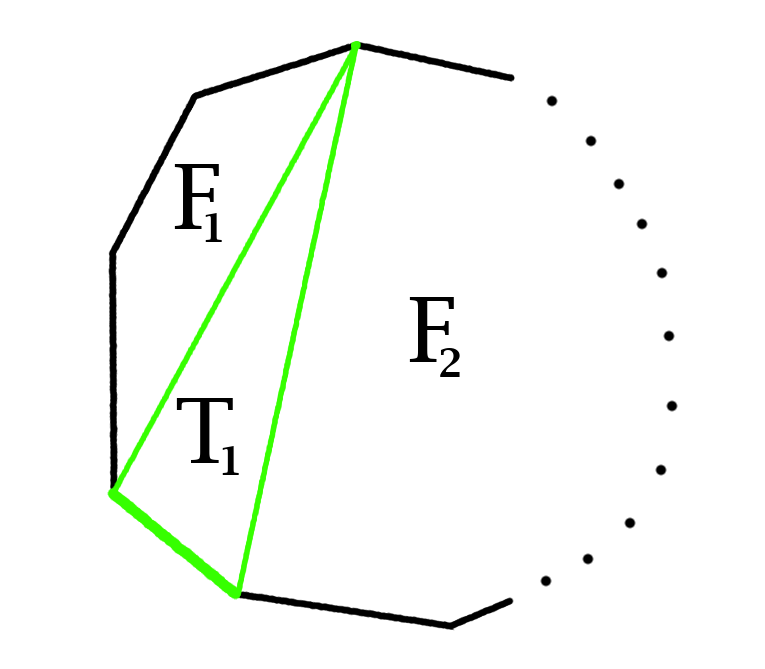
\includegraphics[width=0.5\textwidth]{zad1.png}

Figury $F_1$ oraz $F_2$ dzielimy dalej przekątnymi na rozłączne trójkąty, dopóki jest to możliwe. Jeśli rozpoczniemy podział od jednej ze stron wielokąta, będziemy uzyskiwali trójkąt oraz $i-1$ kąt, aż do ukończenia podziału całej figury. Oznaczmy te podziały przez $q_i$, wtedy liczbę możliwości podziału $n+2$-kąta wyraża wzór:
\[ q_{n+2} = q_{n+1} \cdot q_2 + q_{n} \cdot q_3 + q_{n-1} \cdot q_4 + \ldots + q_3 \cdot q_{n} + q_2 \cdot q_{n+1} \]

Można zauważyć, że po przeindeksowaniu $q_{n+2}$ o $2$ uzyskamy $C_n$, będący liczbą Catalana. Prościej mówiąc, szukana zależność to $q_{n+2} = C_n$, co należało udowodnić.


\section{Zadanie 2}
Przez $x_n$ oznaczmy liczbę drzew binarnych o $n$ wierzchołkach wewnętrznych.

Pojedynczy wierzchołek jest jedynym pełnym drzewem binarnym bez węzłów wewnętrznych, a więc $x_0 = 1$. Mając drzewo $T$ z co najmniej jednym wierzchołkiem wewnętrznym, możemy je jednoznacznie rozłożyć na dwa poddrzewa: lewe $T_L$ oraz prawe $T_R$. Oznaczmy przez $T_n$ rodzinę wszystkich drzew binarnych z $n$ węzłami wewnętrznymi oraz przez $T_{l, r}$ rodzinę wszystkich drzew, których podrzewa $T_L$ oraz $T_R$ mają odpowiednio $l$ oraz $r$ węzłów wewnętrznych. Wtedy mamy:
$abs{T_{l, r}} = \abs{T_l \times T_r} = \abs{T_l} \cdot \abs{T_r} = x_l \cdot x_r$

Zauważmy, że w lewym poddrzewie możemy mieć $0$ wierzchołków wewnętrznych, a w prawym $n-1$ (po rozdzieleniu względem wierzchołka wewnętrznego) lub $1$ w lewym i $n-2$ w prawym, itd. Sytuację taką możemy opisać jako sumę odpowiednich rodzin (zbiorów):
$T_n = T_{0, n - 1} \cup T_{1, n - 2} \cup T_{2, n - 3} \cup \ldots \cup T_{n-1, 0}$
a po wcześniejszym przekształceniu ($\abs{T_{l, r}} = x_l \cdot x_r$), jako następującą sumę:
$x_n = x_0 \cdot x_{n-1} + x_1 \cdot x_{n-2} + \ldots + x_{n-1} \cdot x_0 = C_n$
Oznacza to, że istnieje $C_n$ drzew binarnych o $n$ wierzchołkach wewnętrznych.
\section{Zadanie 3}
Ile niekrzyżujących się uścisków dłoni może wykonać jednocześnie $n$ par osób siedzących za okrągłym stołem? 

Mamy $2n$ osób wykonujących jednocześnie $n$ nieprzecinających się uścisków dłoni. Ponumerujmy te osoby od $1$ do $2n$, aby precyzyjniej mówić o możliwych uściskach. Załóżmy więc, że osoba $1$ wybiera osobę $i$, wtedy pozostałe osoby $2, \ldots, i - 1$ oraz $i + 1, \ldots, 2n$ $\textbf{muszą}$ tworzyć konfigurację, w której  również będą mogły uścisnąć dłonie bez przecięć, a więc żadna osoba nie będzie odizolowana od reszty. Łatwo wywnioskować, że $i$ musi być parzyste, weźmy więc $i = 2k$. 

Wnioskowanie to przypomina problem nawiasowania. Ściślej, mamy do czynienia z $2n$ osobami (nawiasami) oraz $n$ uściskami (dobre pary nawiasów). Aby łatwiej mówić o uściskach, weźmy osoby $i, j$, a następnie podzielmy je sobie na uściski "wychodzące" dla $i < j$ oraz uściski "przychodzące" w przeciwnym przypadku. Uściski wychodzące oznaczać będziemy lewym nawiasem, a przychodzące - prawym. 

Numerując wtedy osoby na okręgu od $1$, która pierwsza wyciąga rękę (uścisk wychodzący), nasz ciąg będzie zaczynał się lewym nawiasem, w przeciwnym wypadku mielibyśmy ciąg nawiasów rozpoczynający się od prawego nawiasu, co nie byłoby poprawne. Przykładowe odzworowanie przedstawiają poniższe rysunki.

(3 RYSUNKI DLA 6 OSOB)
(1-2, 3-4, 5-6) (cieciwy)   
(1-6, 2-5, 3-4) (przekatne)
(1-4, 2-3, 6-5) (pionowe)

Nawiasowaniem dla ustawienia czerwonego będzie $()()()$, dla zielonego $((()))$, a dla niebieskiego $(())()$. Można dostrzec, że im bardziej są od siebie oddalone (w sensie indeksów) osoby, tym więcej nawiasów odzwierciedlających uściski znajdzie się pomiędzy nimi.\\

Opisane wyżej odzworowanie jest bijekcją, dzięki czemu niekrzyżujących się uścisków dłoni dla $2n$ osób jest tyle samo, co dobrych nawiasowań dla $2n$ nawiasów. Jest to $n$-ta liczba Catalana wyrażona wzorem:
$ C_n = \sum\limits_{i = 1}^{n} c_{i - 1} \cdot c_{n - i}$

\section{Zadanie 4}
Ilość drzew binarnych
\section{Zadanie 5}
$a_n = 2*a_{n-1} + 1$
Ciąg $\sequence{a_n}$ jest połączeniem dwóch ciągów:
$\sequence{b_n} = \sequence{2,4,8,16,32,\ldots}$
$\sequence{c_n} = \sequence{-1, -1, -1, -1, -1, \ldots}$
Ciąg $\sequence{b_n}$ to oczywiście ciąg potęg dwójki przesunięty o 1 w lewo. 
Ciąg dwójek wyraża się 
$\frac{1}{1-2x}$, a przesunięcie o k miejsc w lewo:
$\frac{A(x) - (a0x^0+a1x^1+\ldots+a_{k-1}x^{k-1})}{x^k}$
Mamy więc:
$\sequence{b_n} = \frac{\frac{1}{1-2x} - 1x^0}{x^1} = \frac{\frac{1-1+2x}{1-2x}}{x} = \frac{\frac{2x}{1-2x}}{x} = \frac{2}{1-2x}$
Ciąg $\sequence{c_n}$ to ciąg -1.
$\sequence{c_n} = (-1) * \frac{1}{1-x} = \frac{1}{x-1}$

$\sequence{a_n} = \sequence{b_n} + \sequence{c_n} = \frac{2}{1-2x} + \frac{1}{x-1} = \frac{1}{2x^2-3x+1}$

\section{Zadanie 6}
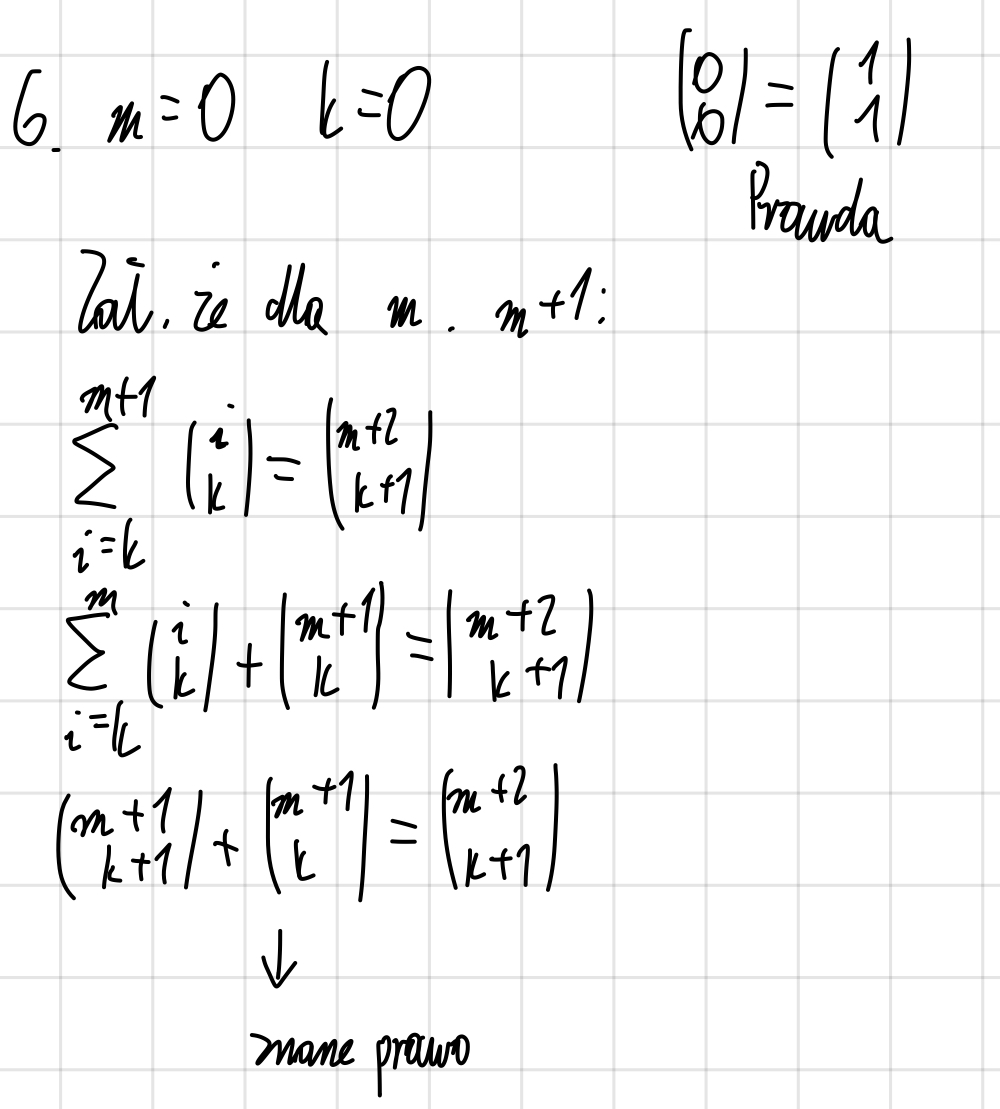
\includegraphics[width=120mm]{zad6}

\section{Zadanie 7}
Mamy pokazać, że dwie kolejne liczby Fibonacciego są względnie pierwsze i powinniśmy skorzystać z algorytmu Euklidesa. 
Wiemy, że kolejnymi wyrazami ciągu Fibonacciego są $F_1 = 1, F_2 = 1, F_3 = 2, \dots$, a kolejne wyrazy są zdefiniowane wzorem $F_{n} = F_{n-1} + F_{n-2}$. Możemy więc indukcyjnie po $n$ (dla $F_n$) udowodnić twierdzenie z zadania.
Podstawa indukcji: $n = 1$, wtedy $\gcd(F_1, F_2) = \gcd(1, 1) = 1$. $\checkmark$ 
Krok indukcyjny: załóżmy, że dla $n$ zachodzi $\gcd(F_n, F_{n+1}) = 1$, pokażemy, że dla $n+1$ zachodzi $\gcd(F_{n+1}, F_{n+2}) = 1$:

$\gcd(F_{n+1}, F_{n+2})	= \gcd(F_{n+1}, F_{n} + F_{n+1}) = \gcd(F_{n+1}, F_{n}) = \gcd(F_{n}, F_{n+1}) = 1$					

\section{Zadanie 8}
1. Jedyną indukcje która da się użyć jest tu:
$NWD(f_n, f_{n-1}) = 1$
Załóżmy, że dla n zachodzi. n+1:
$NWD(f_{n+1}, f_n) = 1$
$NWD(f_n + f_{n-1}, f_n) = 1$
Z wzoru $NWD(n,m)=NWD(n,m+n)$
$NWD(f_{n-1}, f_n) = 1$
Podstawa indukcji więc udowodnione.

2. Jeśli NWD(m, n) = 1 to NWD(m, nk) = NWD(m, k)
3. $f_{m+n} = f_mf_{n+1} + f_{m-1}f_n$
Indukcja po n. Dla n=0:
$f_m = f_mf_1 + f_{m-1}f_0 = f_m$
Założenie: $f_{m+n} = f_mf_{n+1} + f_{m-1}f_n$
n+1:
$f_{m+n+1} = f_mf_{n+2} + f_{m-1}f_{n+1}$
$f_{m+n} + f_{m+n-1}  = f_mf_{n+1} + f_mf_{n}  + f_{m-1}f_{n} + f_{m-1}f_{n-1}$
$f_{m+n-1} = f_mf_{n} + f_{m-1}f_{n-1}$
Niech k = n+1 
$f_{m+k} = f_mf_{k+1} + f_{m-1}f_k$
Co jest założeniem indukcyjnym.
Także zachodzi.


Niech $n = mk+r$, gdzie $0 \leq r < m$
$NWD(f_m, f_n) = NWD(f_m, f_{mk+1}f_r + f_{mk}f_{r-1})$ z lematu 3
$NWD(f_m, f_{mk+1}f_r + f_{mk}f_{r-1}) = NWD(f_m, f_{mk+1}f_r)$ bo $f_m|f_{mk}$
$NWD(f_m, f_{mk+1}f_r) = NWD(f_m, f_r)$ z lematu 2
Powyższy wzór jest wzorem na algorytm euklidesa. 
Niech $NWD(m,n) = s$
Także wynikiem $NWD(f_m, f_n) = NWD(f_s, 0) = f_s = f_{NWD(m, n)}$



\section{Zadanie 9}
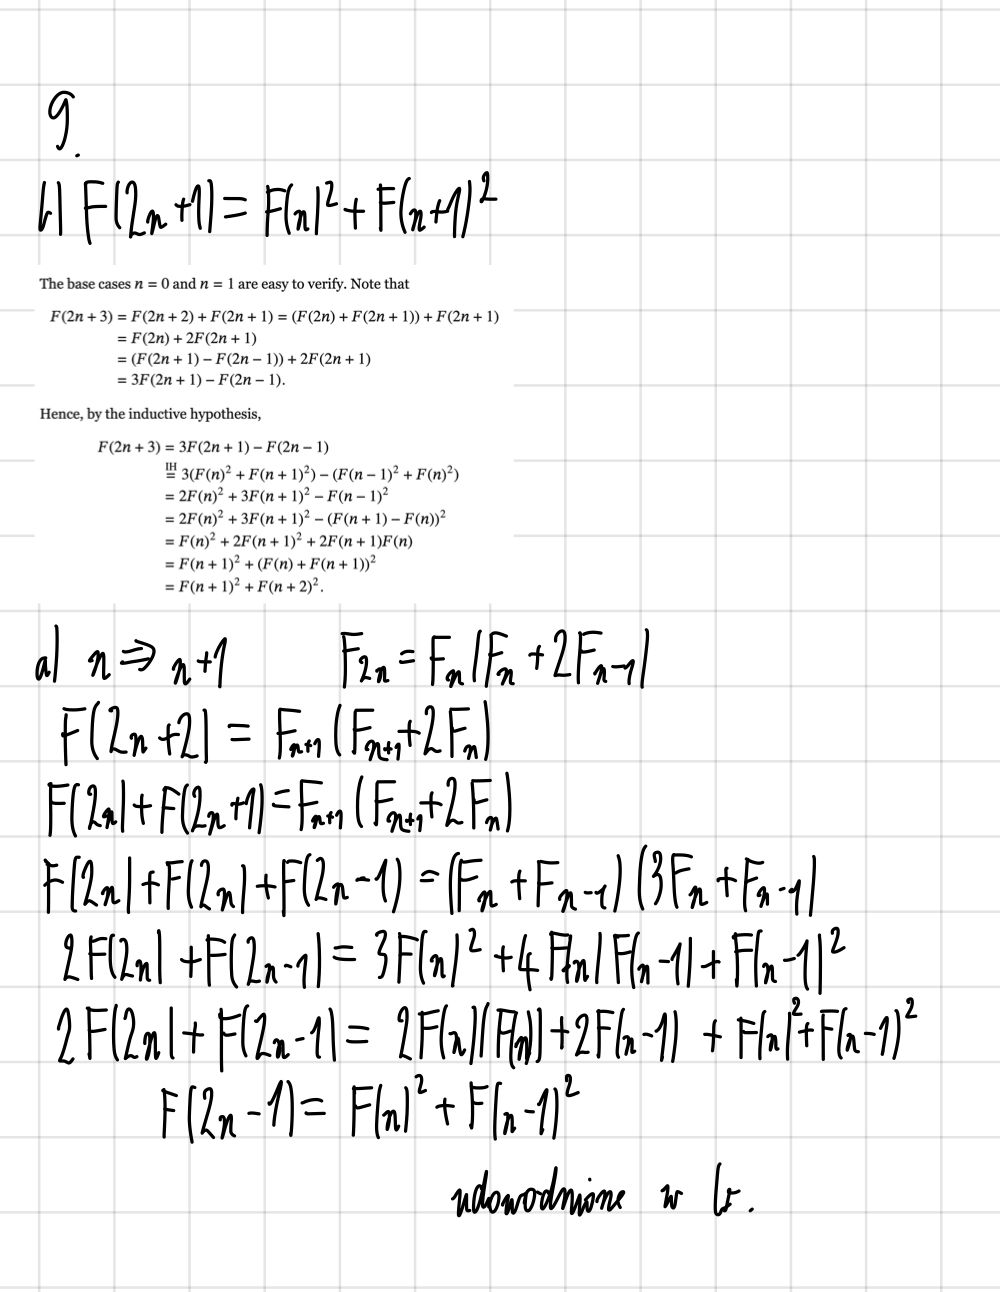
\includegraphics[width=120mm]{zad9}

\section{Zadanie 10}
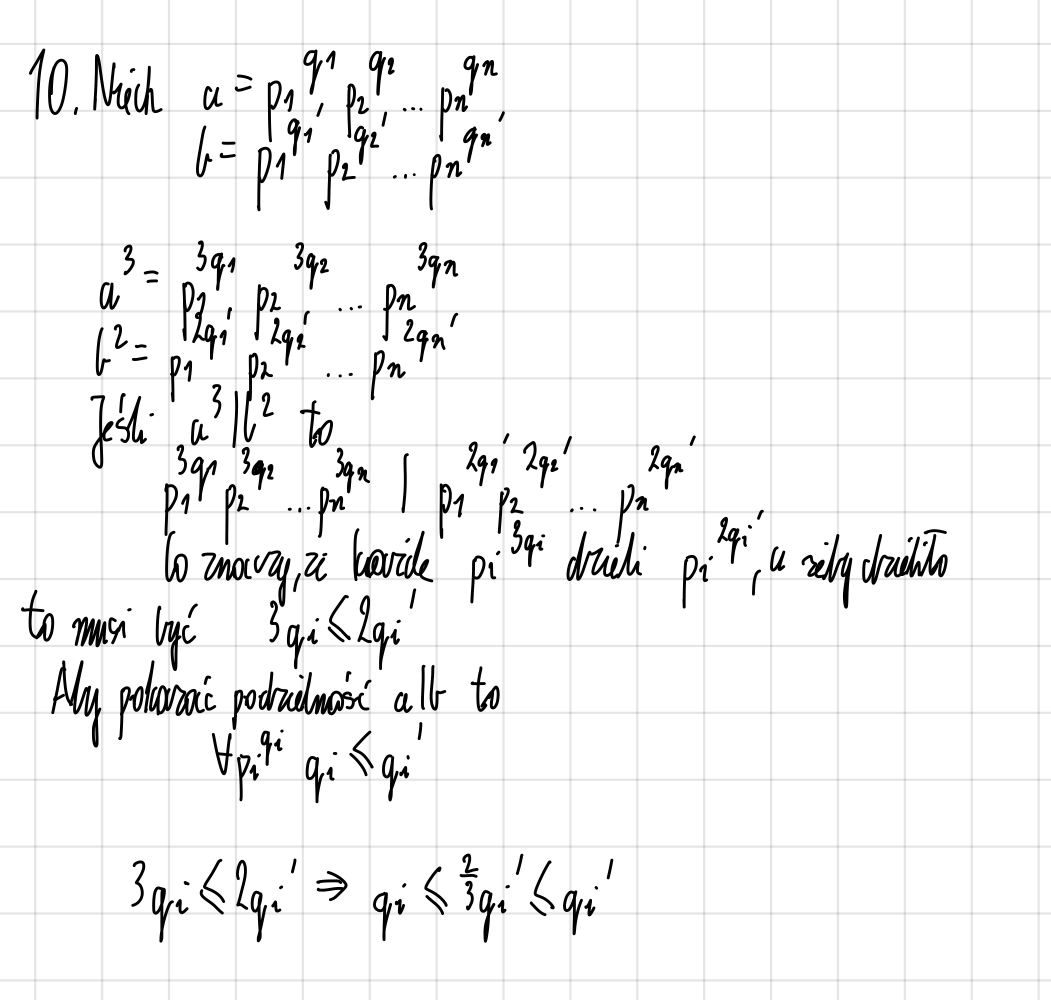
\includegraphics[width=120mm]{zad10}

\egroup
\end{document}